%%%%%%%%%%%%%%%%%%%%%%%%%%%%%
%% Event reweighting 
%%%%%%%%%%%%%%%%%%%%%%%%%%%%%

\subsubsection{Pileup reweighting \label{sec:event_pileup}}

The distribution of the number of pileup interactions is different in data with respect to
simulation. Given that the number of pileup interactions can have an influence on various aspects of
the reconstruction, such as the identification of primary vertices or lepton isolation, 
the simulated events should be reweighted such that their pileup distribution matches that of
data~\cite{pileup_twiki}.

The pileup distribution in data is provided centrally by the Physics Validation Group for each
data taking period. This distribution depends on the total $\Pp\Pp$ inelastic cross section. 
In simulation, the pileup distribution is taken from truth information, through the variable
\texttt{trueNumInteractions} which stores how many pileup events were overlaid on the hard scatter. 
The pileup weights are computed as the ratio of the normalized pileup distributions in data and
simulation, and should be applied to all simulated events.
The distribution of the pileup in data and simulation, and the corresponding pileup weight is
shown in Figure~\ref{fig:pileup_comparison}. As can be seen, the initial guess for the pileup
distribution, which was implemented in the simulation, was not perfect, resulting in an effective
reduction of the statistical precision of the simulated samples. 

\begin{figure}[htpb]
 \centering
 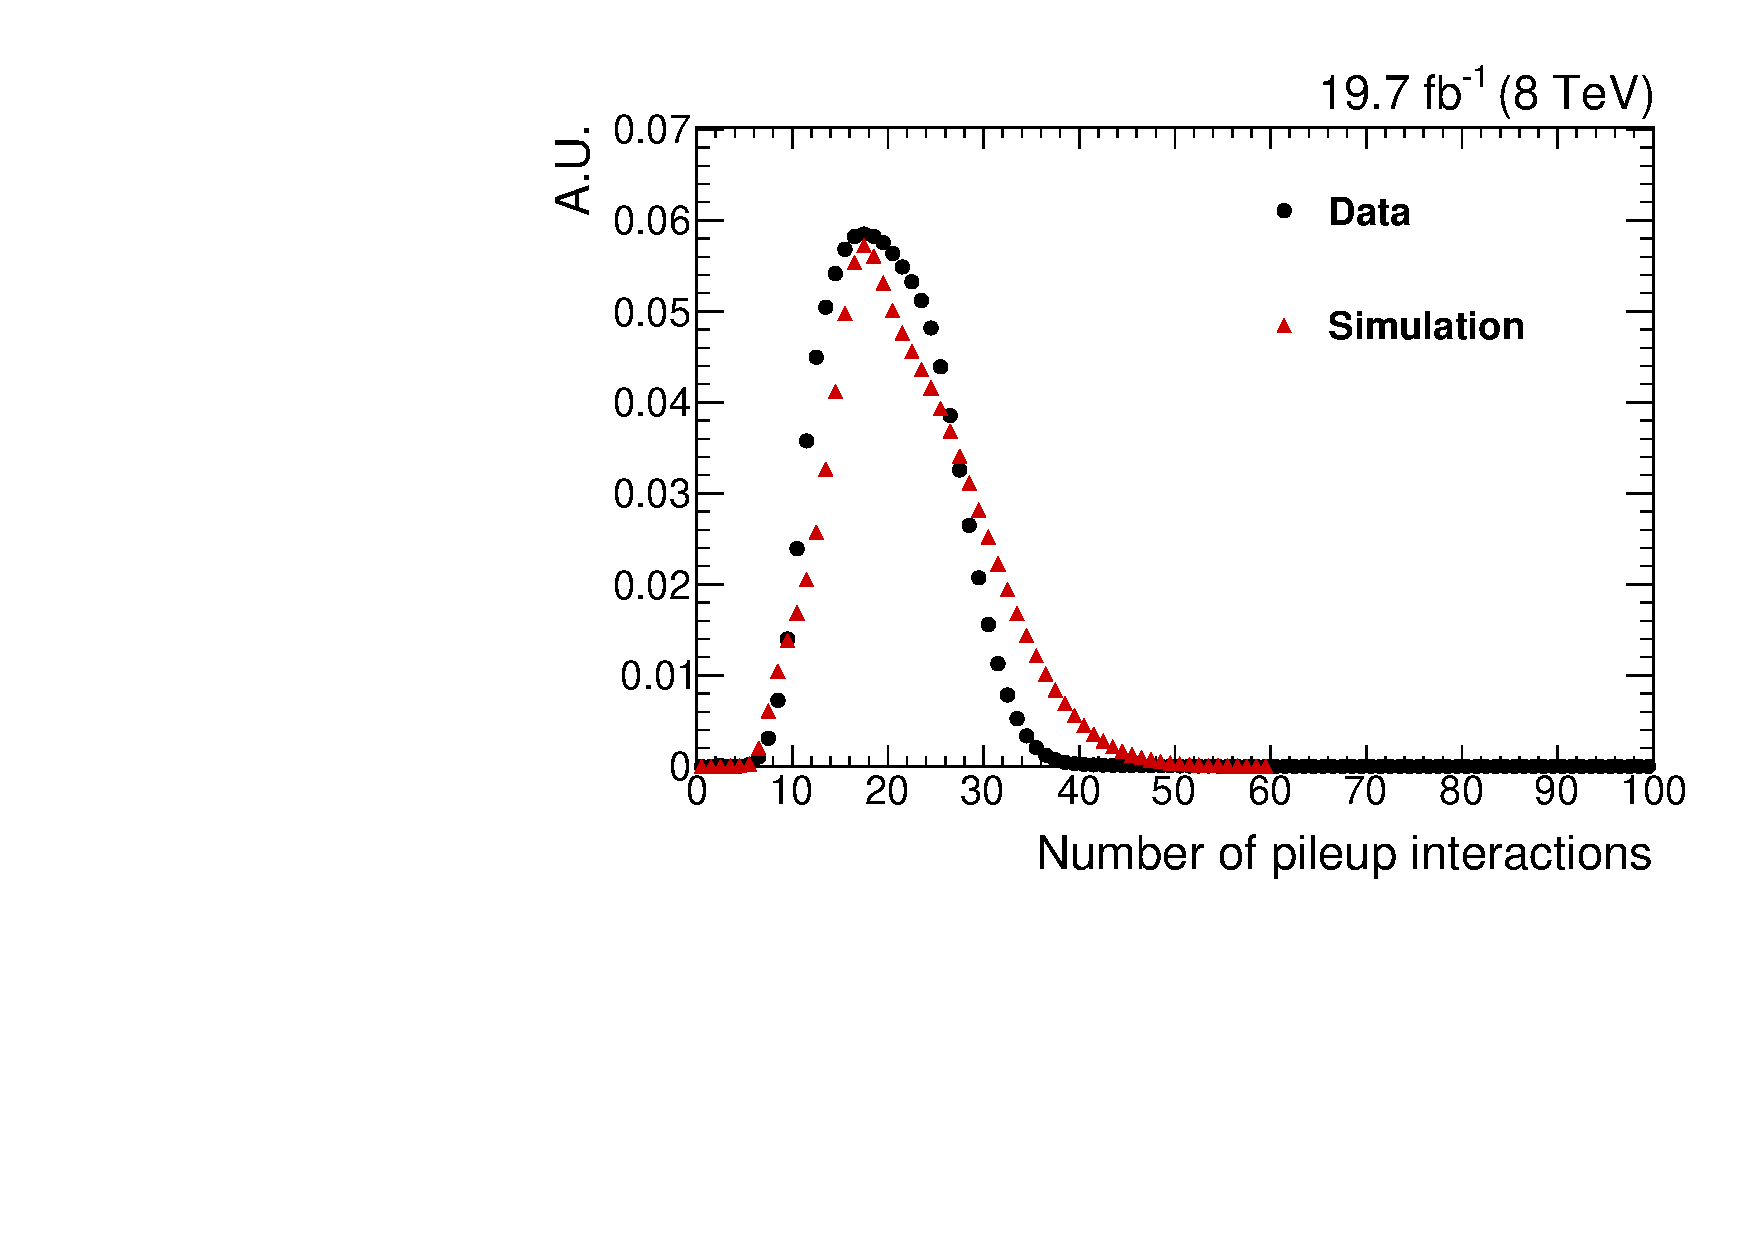
\includegraphics[width=0.48\textwidth]{figures/eventreco_reweighting/pileup_comparison}
 ~
 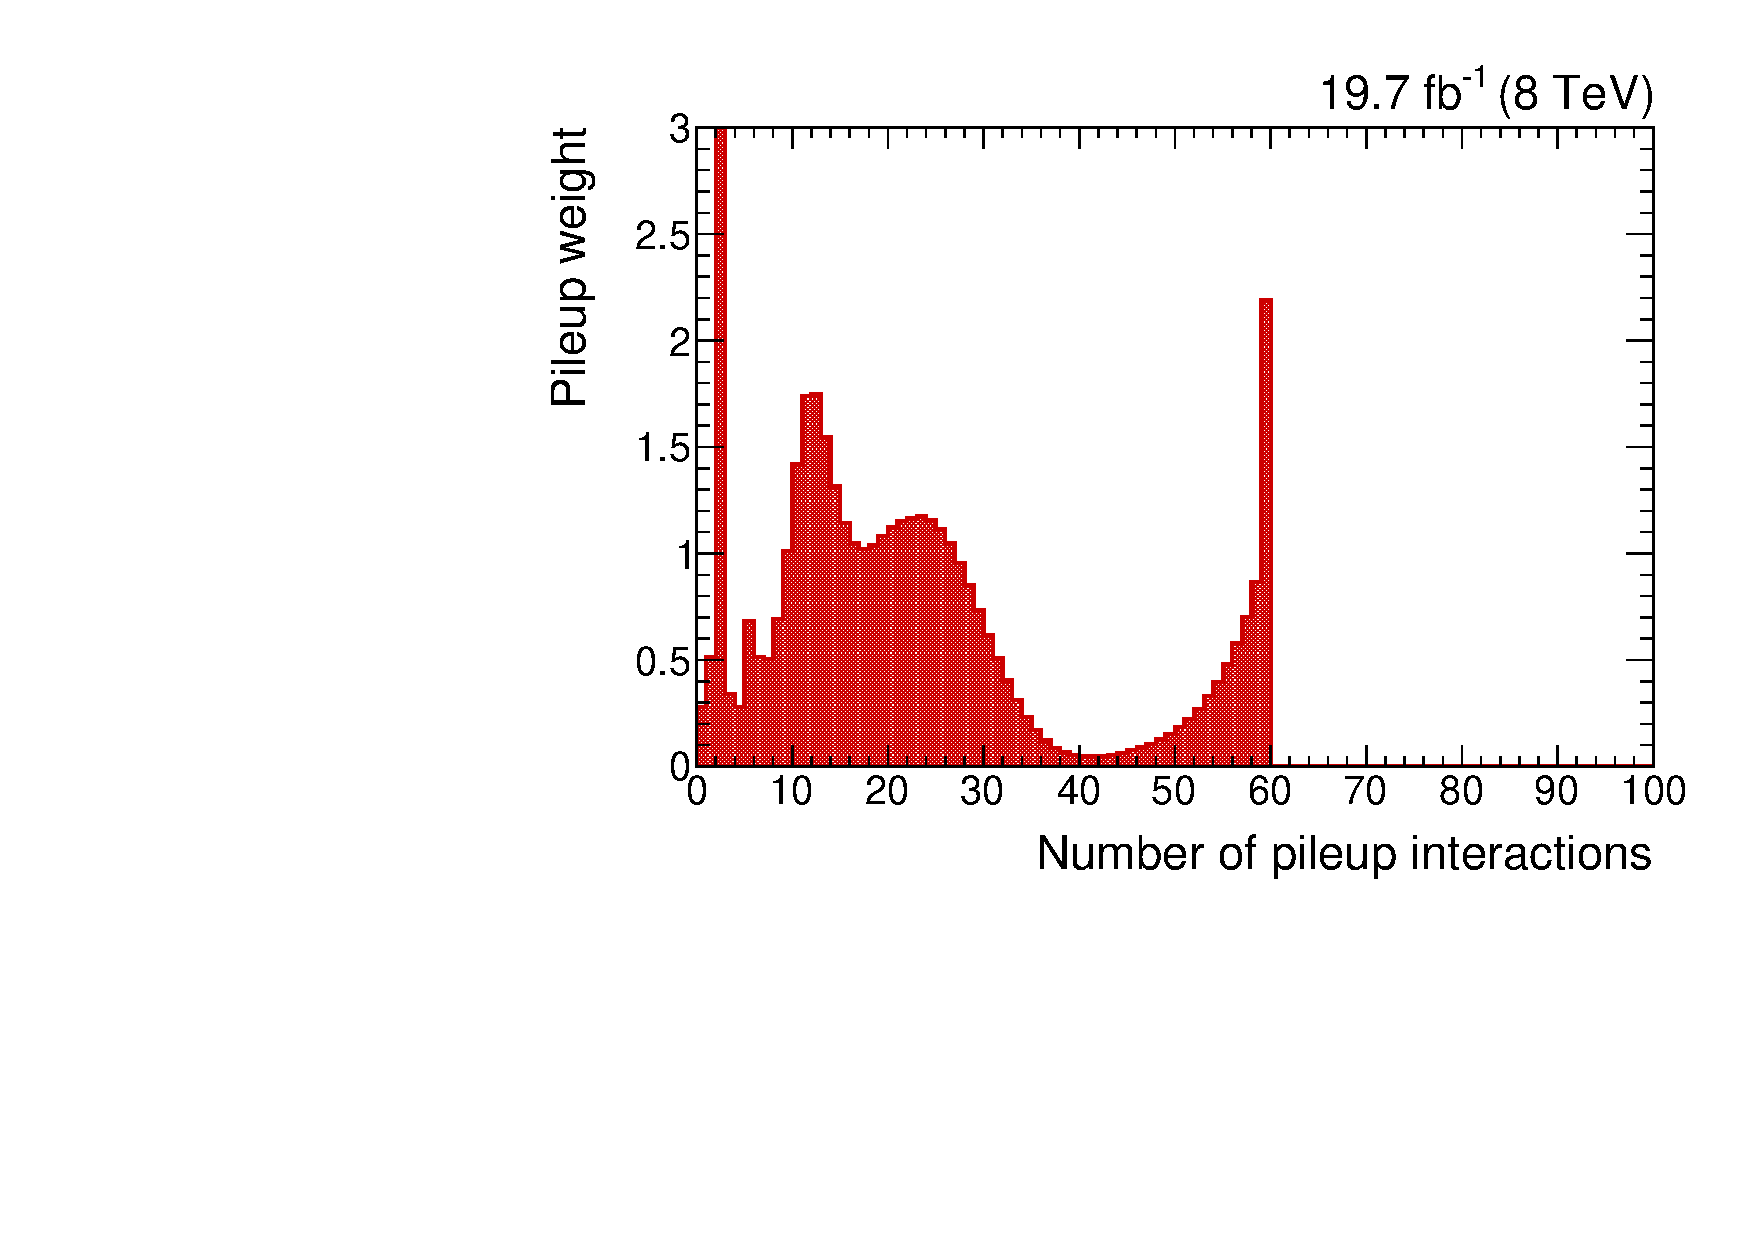
\includegraphics[width=0.48\textwidth]{figures/eventreco_reweighting/pileup_weight_comparison}
\caption{[left] Comparison of the distribution of the number of pileup interactions in data and in
simulation. 
[right] Pileup weight as a function of the number of interactions. 
\label{fig:pileup_comparison}}
\end{figure}

% TODO decide whether to add the data mc comparison for the primary vertices

% 
% As a test of the performance of the pileup reweighting, we can check the agreement between data
% and
% simulation for the distribution of the number of good primary vertices ($PV$) at different
% selection
% levels. 
% We expect to find a reasonable, although not perfect agreement as the vertex reconstruction
% efficiency depends on many things. 
% This comparison is shown in figure~\ref{fig:comparison_PV}. 
% 
% \begin{figure}
%  \includegraphics[width=0.49\textwidth]{figures/Pileup/DataMC_PV_0Lb1Ll}
%  \includegraphics[width=0.49\textwidth]{figures/Pileup/DataMC_PV_g1Mb1Ll}
% \caption{Data/MC comparison plot of the number of good primary vertices after pileup reweighting
% for
% a control region enhanced in $W+$jets (left) and enhanced in $t\bar{t}+$jets (right).
% \label{fig:comparison_PV}}
% \end{figure}
% 


\subsubsection{ISR reweighting \label{sec:event_ISRreweighting}}

Searches for new physics often rely on an initial state boost of the produced system in order to
have experimental acceptance for the signature under consideration. This is especially important
for models featuring a compressed mass spectrum. A high-\pt ISR jet can be used to suppress
background, or the boost can raise the momentum of jets or leptons in the decay chain to a level
that is detectable.
A mismodelling of the initial state radiation, or uncertainty on the modelling, will thus
directly impact the interpretation of these searches. 

A study was performed to investigate how well the ISR is
modelled in the simulation by evaluating the agreement between data and simulation in the boost \pt
for $\cPZ+$jets and $t\bar{t}$ events~\cite{Chatrchyan:2013xna,ISRreweighting}. 
For $\cPZ+$jets events the boost \pt was measured from the leptonic decay products of the $\cPZ$
boson. For $t\bar{t}$ events the ISR radiation was measured using the hadronic recoil system, which
is computed from all jets except for the $\cPqb$-tagged jets from the $t\bar{t}$ decay. 

It was found that the initial state radiation is not well modelled at high \pt, as illustrated in
Fig.~\ref{fig:ISRreweighting}. The mismodelling
can be corrected by applying a scale factor, with associated uncertainty, which was derived from the
observed disagreement. The scale factor depends on the \pt of the system recoiling against the ISR
jets. This system could be e.g. the $t\bar{t}$ system, the $\cPZ$ boson, or the $\tilde{g}\tilde{g}$
system for a SUSY event.  The uncertainty on this scale factor is taken to be the difference
between the scale factor and unity. 
The CMS SUSY group recommends to apply this ISR reweighting to all SUSY signal samples.
The prescription is summarized in Table~\ref{tab:ISRreweighting}. 

\begin{figure}[tpb]
  \centering
  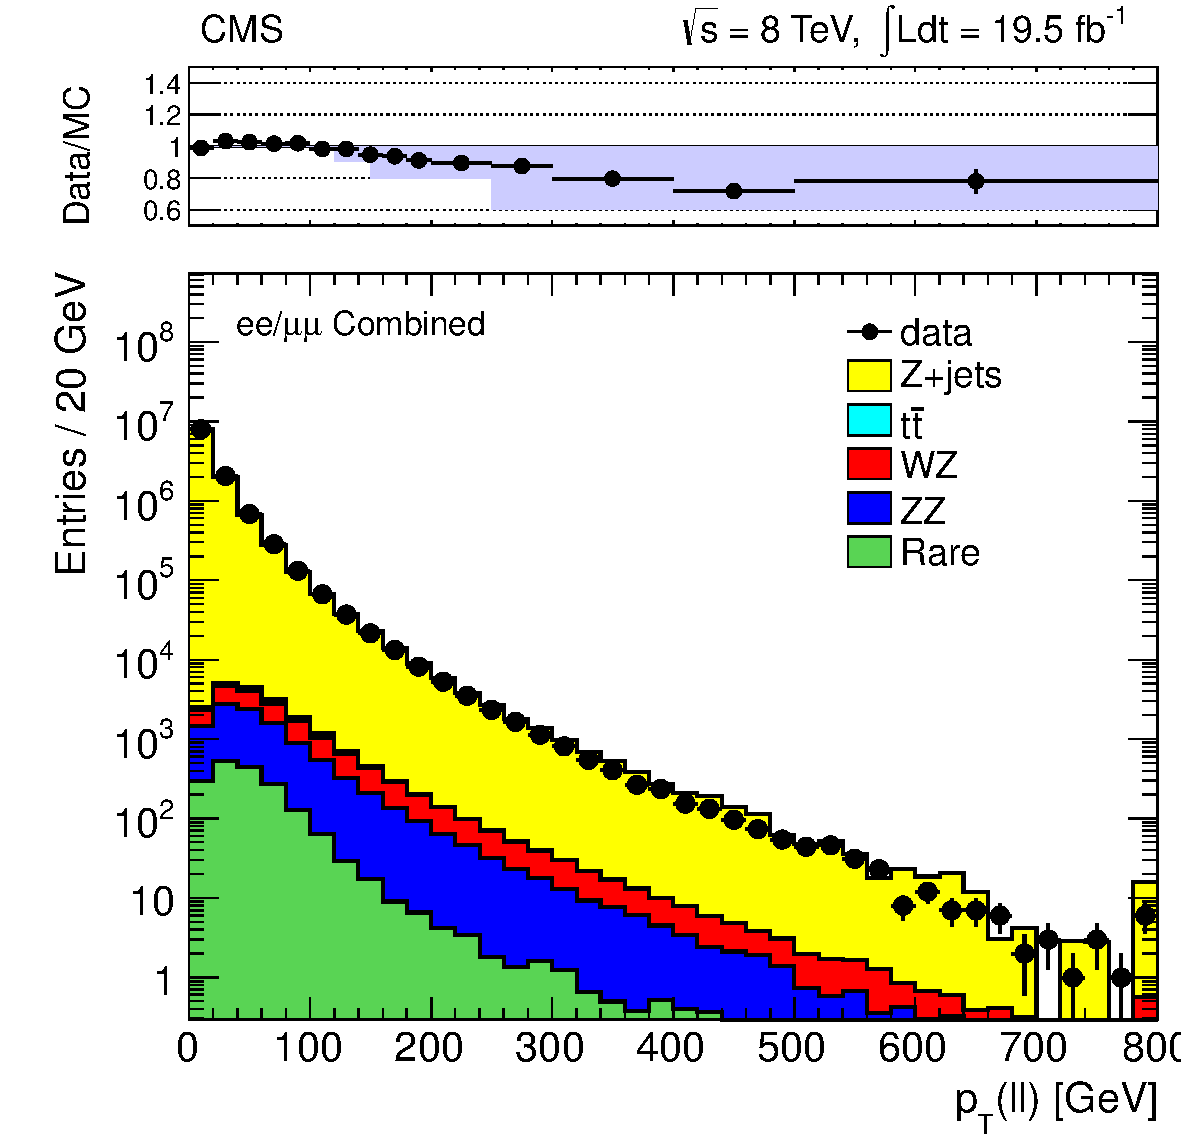
\includegraphics[width=0.7\textwidth]{figures/eventreco_reweighting/ISR_reweighting}
  \caption{ Comparison of data to simulation for the \pt of the dilepton ($ee$ or
$\mu\mu$) system in $\cPZ$+jets events. The prediction from simulation is normalized to the total
data yield to compare the shapes of the distributions. The ratio of data/simulation is shown at the
top of the figure, and the light blue band shows the weights derived for simulation and the
variation to assess systematic uncertainties. Figure from Ref.~\cite{Chatrchyan:2013xna}.
  \label{fig:ISRreweighting}}
\end{figure}

\begin{table}[htpb]
\caption{ISR reweighting prescription. \label{tab:ISRreweighting}}
\begin{center}
\begin{tabular}{c c}
\toprule
\pt of recoiling & Scale factor \\ 
system (\GeV) & \\
\midrule
$\leq 120$ & $1.00 \pm 0.00$ \\
$120 - 150 $ & $0.95 \pm 0.05$ \\
$150-250$ & $0.90 \pm 0.10$ \\
$> 250$ & $0.80 \pm 0.20$ \\
\bottomrule
\end{tabular}
\end{center}
\end{table}




\subsubsection{Top quark \texorpdfstring{$\pt$}{pt} reweighting \label{sec:event_toppt_reweighting}}

Differential top-quark-pair cross section analyses have shown that the shape of the \pt spectrum of 
top quarks in data is softer than predicted by simulation~\cite{toppt,toppt_twiki}. 
To remedy this, events are reweighted based on the \pt of the generator level $t$ and $\bar{t}$
quarks in the $t\bar{t}$ simulation.
The event weight, $w_{\rm TopPt}$, is computed as a function of the generated \pt of both the top
and anti-top quark in the event: 
\begin{equation}
w_{\rm TopPt} = \sqrt{ SF_t \cdot SF_{\bar{t}} }
\end{equation}
\begin{equation}
SF(\pt^{gen}) = \exp(a + b\, \pt^{gen})
\end{equation}
with $a = 0.156$ and $b = -0.00137$.
The uncertainty associated with this reweighting is taken to be equal to the full size of the
reweighting, which gives for the one standard deviation up and down variations of the event
weight:
\begin{align}
 +1~\sigma &: w_{\rm up} = w_{\textrm{TopPt}} \cdot w_{\textrm{TopPt}}, \\
 -1~\sigma &: w_{\rm down} = 1 .
\end{align}
The effect of this reweighting on the data/simulation agreement in a $t\bar{t}$ enriched region is
shown in Fig.~\ref{fig:TopPt}. The $x$-axis on these plots shows the razor variable $\mr$, which
will be defined in Section~\ref{sec:boost_razor}. It is clear that including this reweighting
improves the agreement. 

 
\begin{figure}[htpb]
\centering
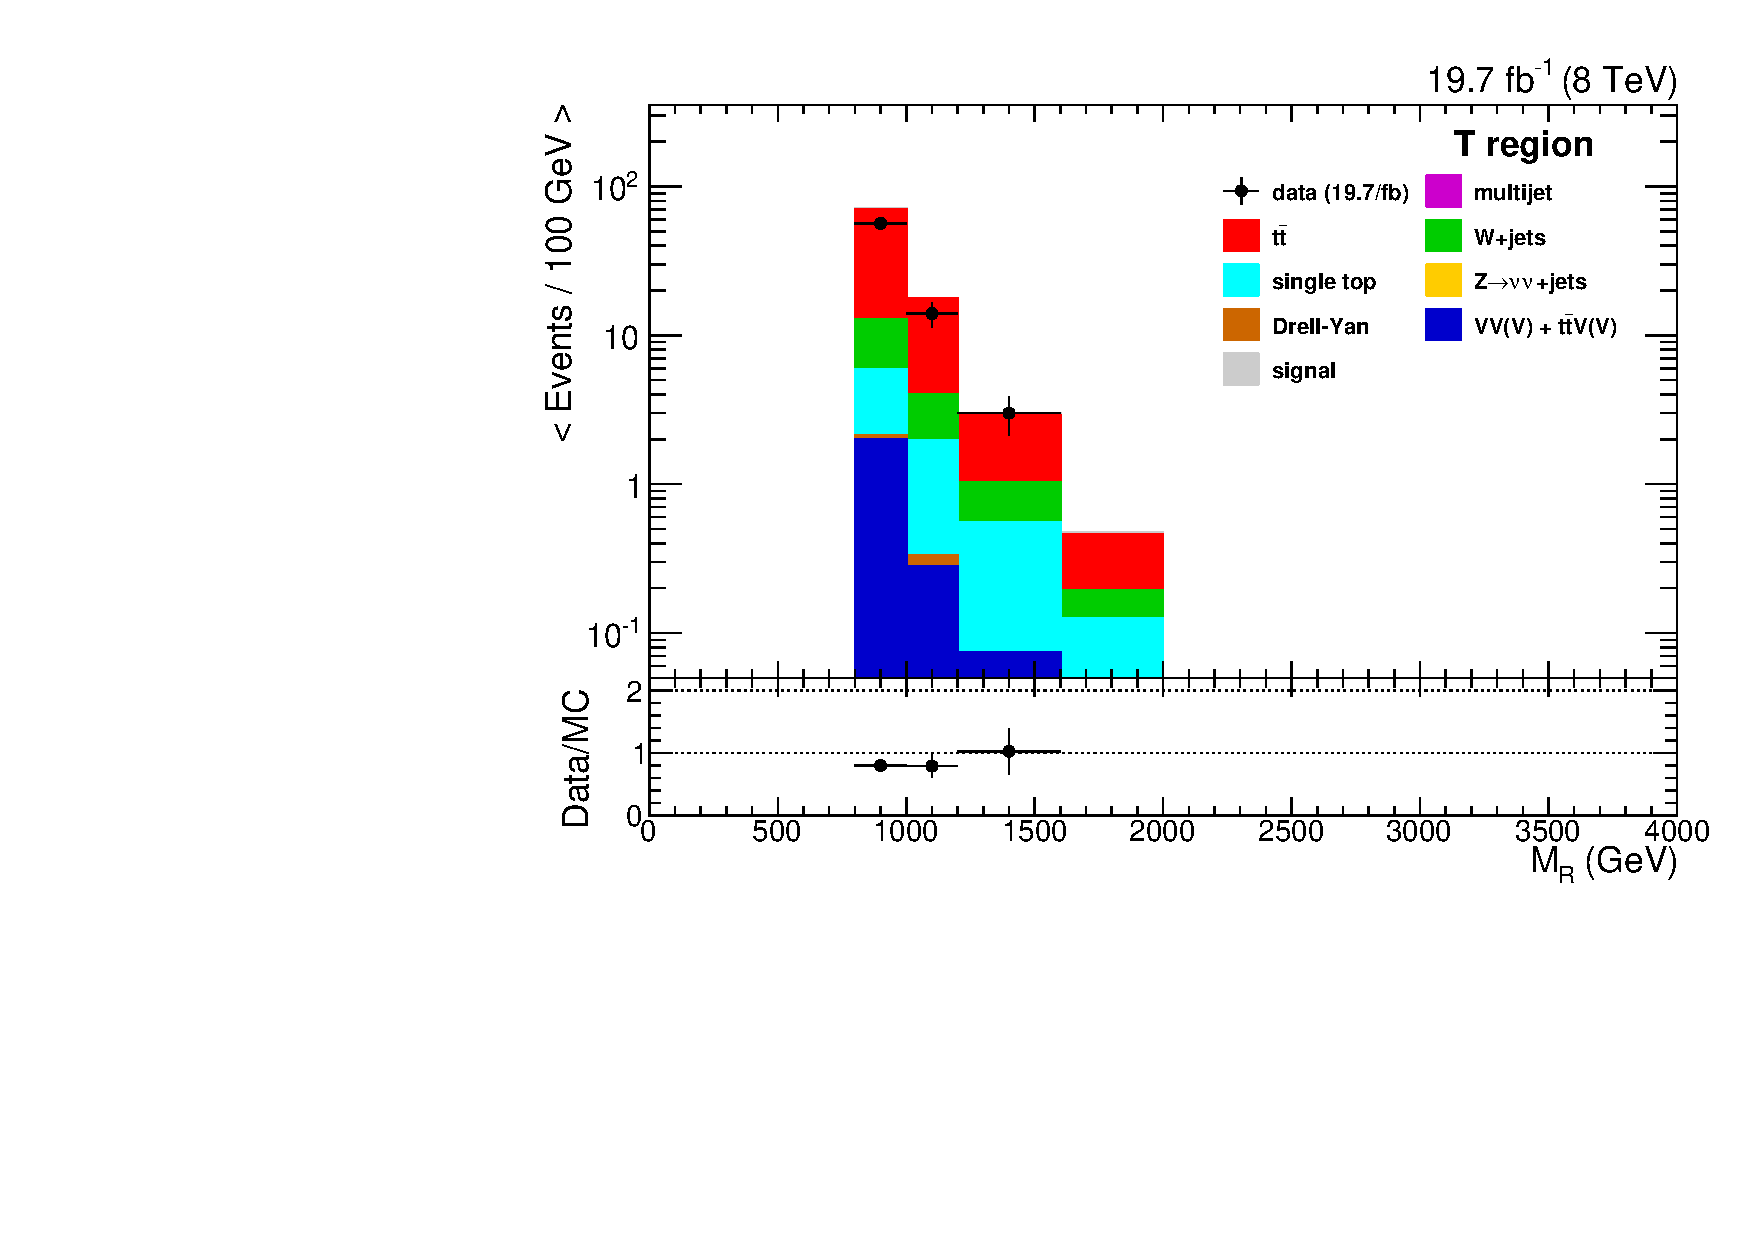
\includegraphics[width=0.48\textwidth]
{figures/razor_selection/plots_noTopPt/DataMC_MR_g1Mbg1W1LlmT100_mdPhig0p5_width}
~
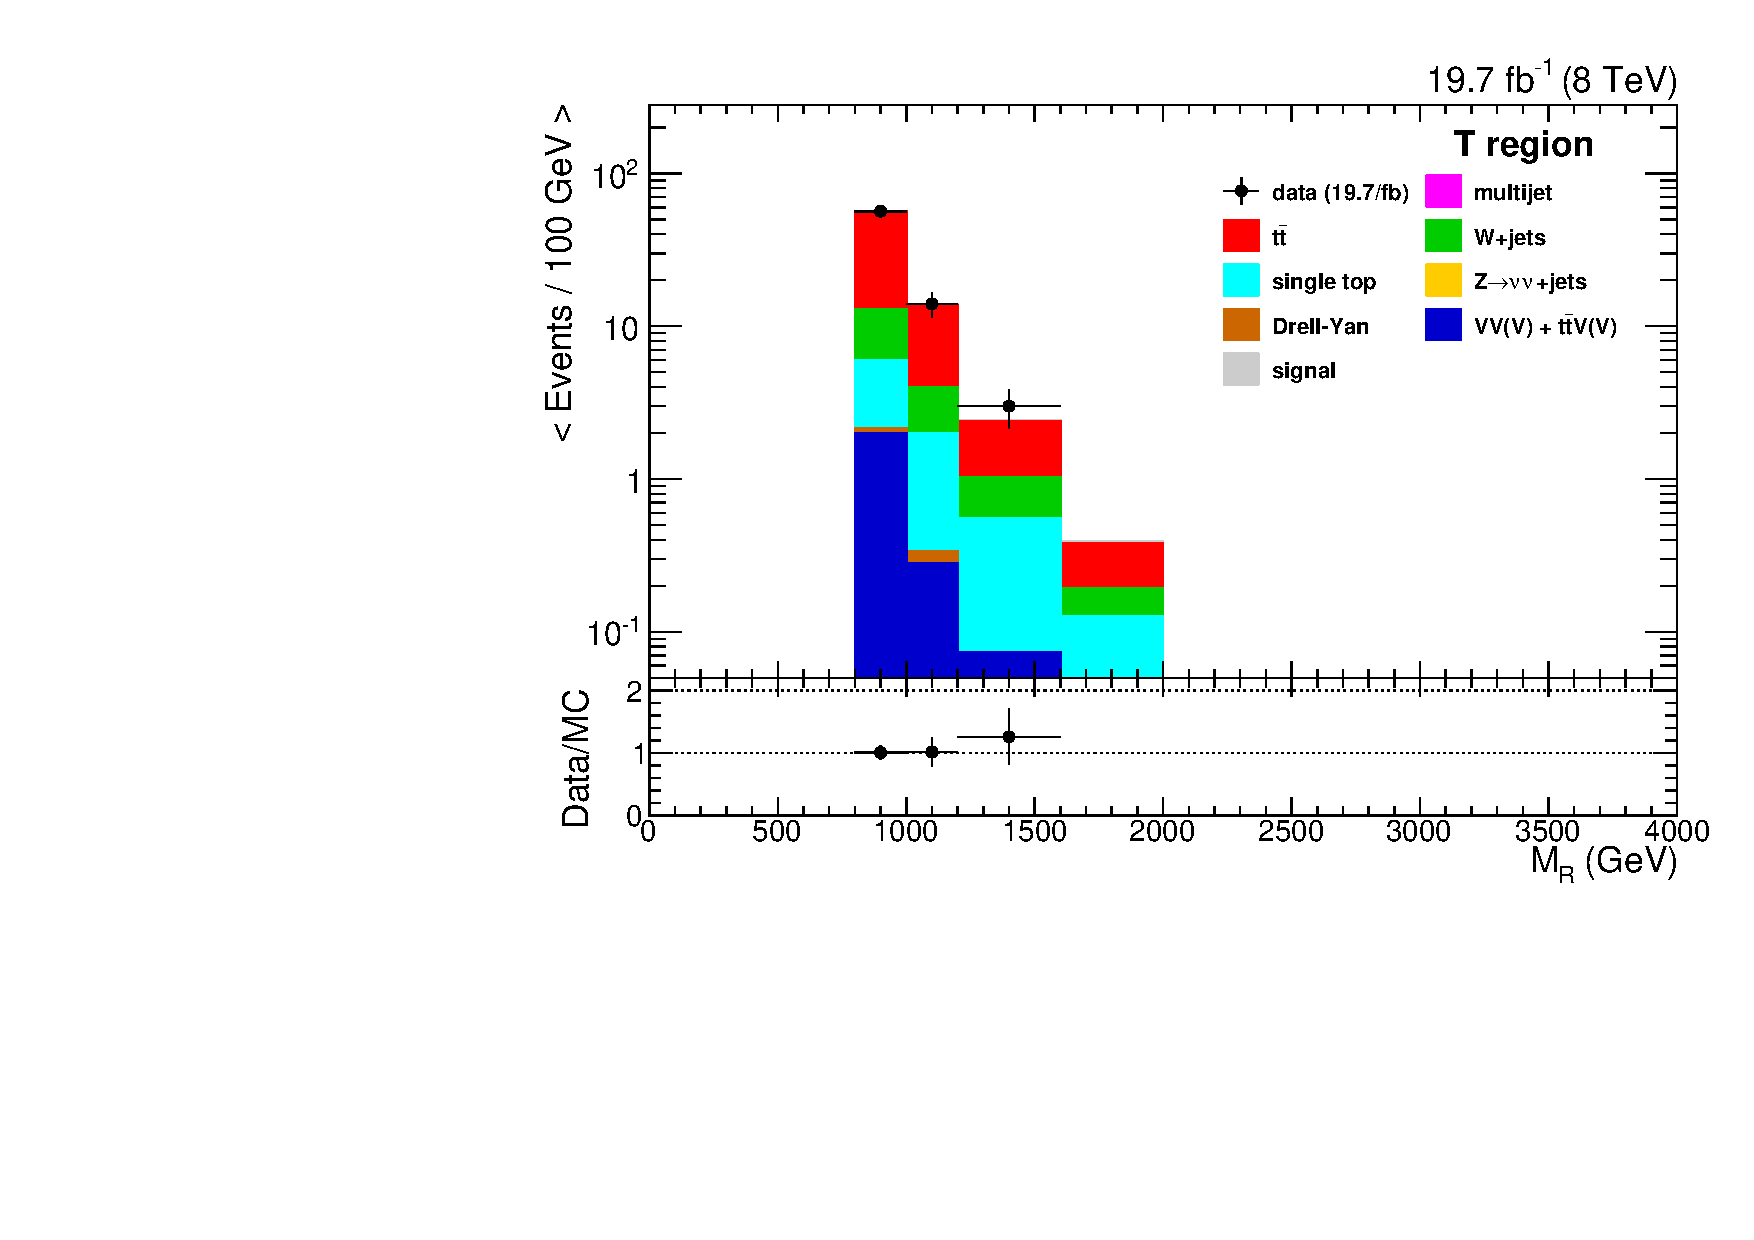
\includegraphics[width=0.48\textwidth]
{figures/razor_selection/plots/DataMC_MR_g1Mbg1W1LlmT100_mdPhig0p5_width}
\caption{Distribution of the razor variable $\mr$ in data and simulation before applying the top
\pt reweighting (left), and after (right). 
\label{fig:TopPt}}
\end{figure}



